\FILE{devops.tex}

\section{System Management}

The goals of FutureGrid to offer a variety of services as part of its
testbed features is going beyond services that are normally offered by
data and supercomputing centers for research. This provides a number
of challenges that need to be overcome in order to efficiently manage
the system and provide services that have never been offered to users
as they exist on FutureGrid.

\subsection{Integration of Systems and Development Team}

FutureGrid started initially with a model where the systems team and
the software team were separated. A clear wall of responsibilities was
erected that resulted in multiple challenges:

\begin{enumerate}

\item
The system setup and management was completely separated from
the software development team focussing mostly on the deployment of
existing technologies. 

\item
The system was complex, but its deployment was documented to a limited
extend not allowing the developers to utilize it properly.

\item 
Lack of trust by the systems team dis not allow the software team to
have a valid development environment.

\item
The software developed needed a testbed within the
testbed that was not necessarily reflecting the actual system setup.

\end{enumerate}

Together these issues, made it extremely difficult if not impossible to
further any development in regards to the design of a testbed
infrastructure as requested by our original ambitious goals. 

To overcome these difficulties it was decided that the systems team
must be integrated in some fashion into the software team and become
part of the development process. This integration is not an isolated
instance within FutureGrid, but is also executed in many modern data
centers and is now recognized with its own term called {\em DevOps}.

\subsection{DevOps}

Devops is not just a buzzword from industry and research communities,
but it provides value added processes to the deployment and
development cycles that are part of modern data centers. It can today
be understood as a software development method that stresses
collaboration and integration between software developers and
information technology professionals such as a system administrator. 

WHile using an infrasrtructure such as clouds we recognized early on
that the lifetime of a particular IaaS framework is about 3-6 month
before a new version is installed. This is a significant difference to
a traditional High Performance Computing Center that is comprised of
many software tools experiencing much longer life spans. This is not
only based on security patches but significant changes for example in
the evolving security, user services as well as the deployment of new
services that become avalable in rapid procession.

This rapid change of the complex infrastructure requires a rethinking
about how systems in general are menaged and how they can be made
avalable to the development teams. While previously it may have been
enough to install updates on the machines, DevOps frameworks provide
the developer and system administarors to create and share
enviroenments that are used in production and development while at the
same time increasing quality assurance by leveraging each others
experiences (see Figure \ref{F:devops}).

\begin{figure}[htb]
  \centering
   \begin{minipage}{.5\textwidth}
    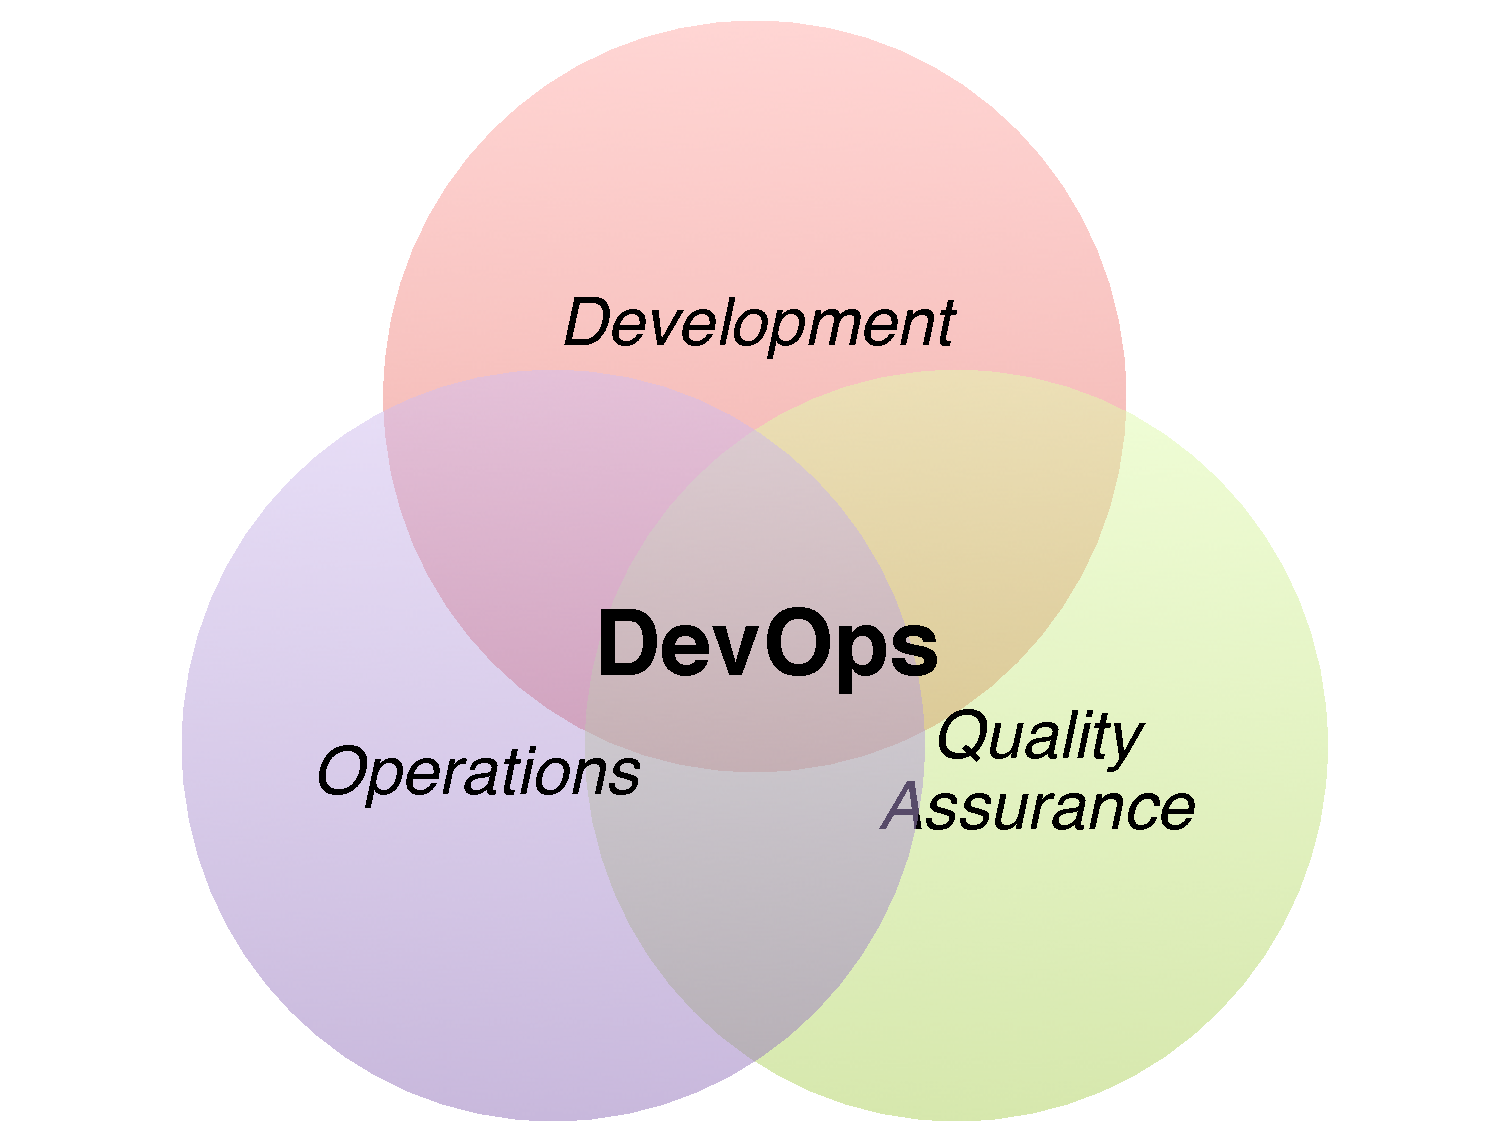
\includegraphics[width=1.0\textwidth]{images/devops.pdf}
    \caption{DevOps Intersection.}
    \label{F:devops}
  \end{minipage}%
   \begin{minipage}{.5\textwidth}
     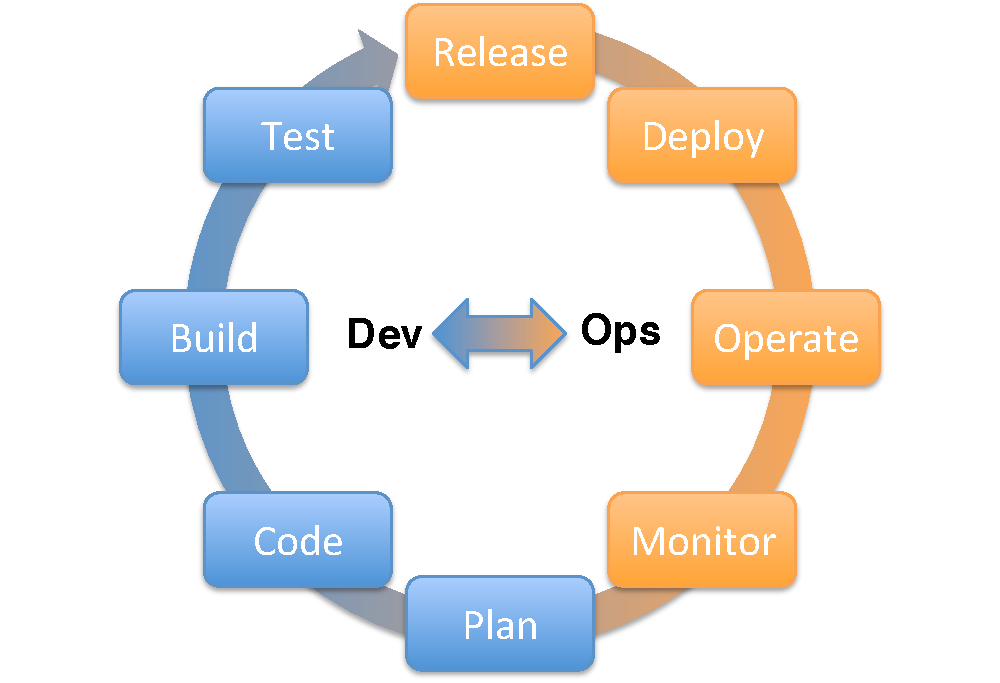
\includegraphics[width=1.0\textwidth]{images/devops-circle.pdf}
     \caption{DevOps Cycle.}
     \label{F:devops-circel}
  \end{minipage}%
\end{figure}

\subsection{DevOps Cycle}

While combining the steps executed by the Development and operational
team from planing, to coding, building and testing, to the release,
deployment and operation and monitoring (see Figure
\ref{F:devops-circle}), each of the phases provides a direct feedback
between the DevOps team members and shortening thus the entire
development phase. It also allows to test out new services and
technologies in a rapid progression. Hence it is possible to roll out
new developments much faster into production. This leads to a much mor
rapid integrated cycle than without the correlation between
development and operation would be possible.

\subsection{DevOps Supporting Tools}

A number of tools are available that make the introduction of DevOps
strategies more efficient. The first is the need for an efficient
communication pathway to manage tasks not only between developers but
also between users. Thus the ideal system would provide a complete
integration of a project management system that allows to manage tasks
for both developers and operators, but also to easily integrate
tickets and transform them into tasks. In XSEDE and other
supercomputing centers a system called RT is typically used for user
ticket management. Other systems such as jira, mantis, and ??? are
often used to manage the software and systems related
tasks. Unfortunately, personal or organizational constraints prevent
often the integration of the two systems and additional overhead is
needed to move user tickets into tasks and the development
cycle. Within FutureGrid we experimented as part of our opensource
development extensively with jira as systems and ticketing system
reveling that newest development in such areas motivated by DevOps
teams lead to tools that support the overall cycle including users
(see Figure \ref{F:usedevops}). However, the integration of
FutureGrid within the overall much larger XSEDE effort did make it not
possible to switch from RT to jira for user ticket
management. To stress this user integration we term this framework
{\em UseDevOps}. Tools to integrate Development and Operation
deployment include puppet, chef, ansible, cfengine and bcfg2. While
FutureGrid started out with bcfg2 we have since than switched to other
tools due to their prevalence within the community. Chef, puppet, and
ansible have significant amount of traction. Due to expertise within
our group we currently explore chef and ansible. 

\begin{figure}[htb]
  \centering
    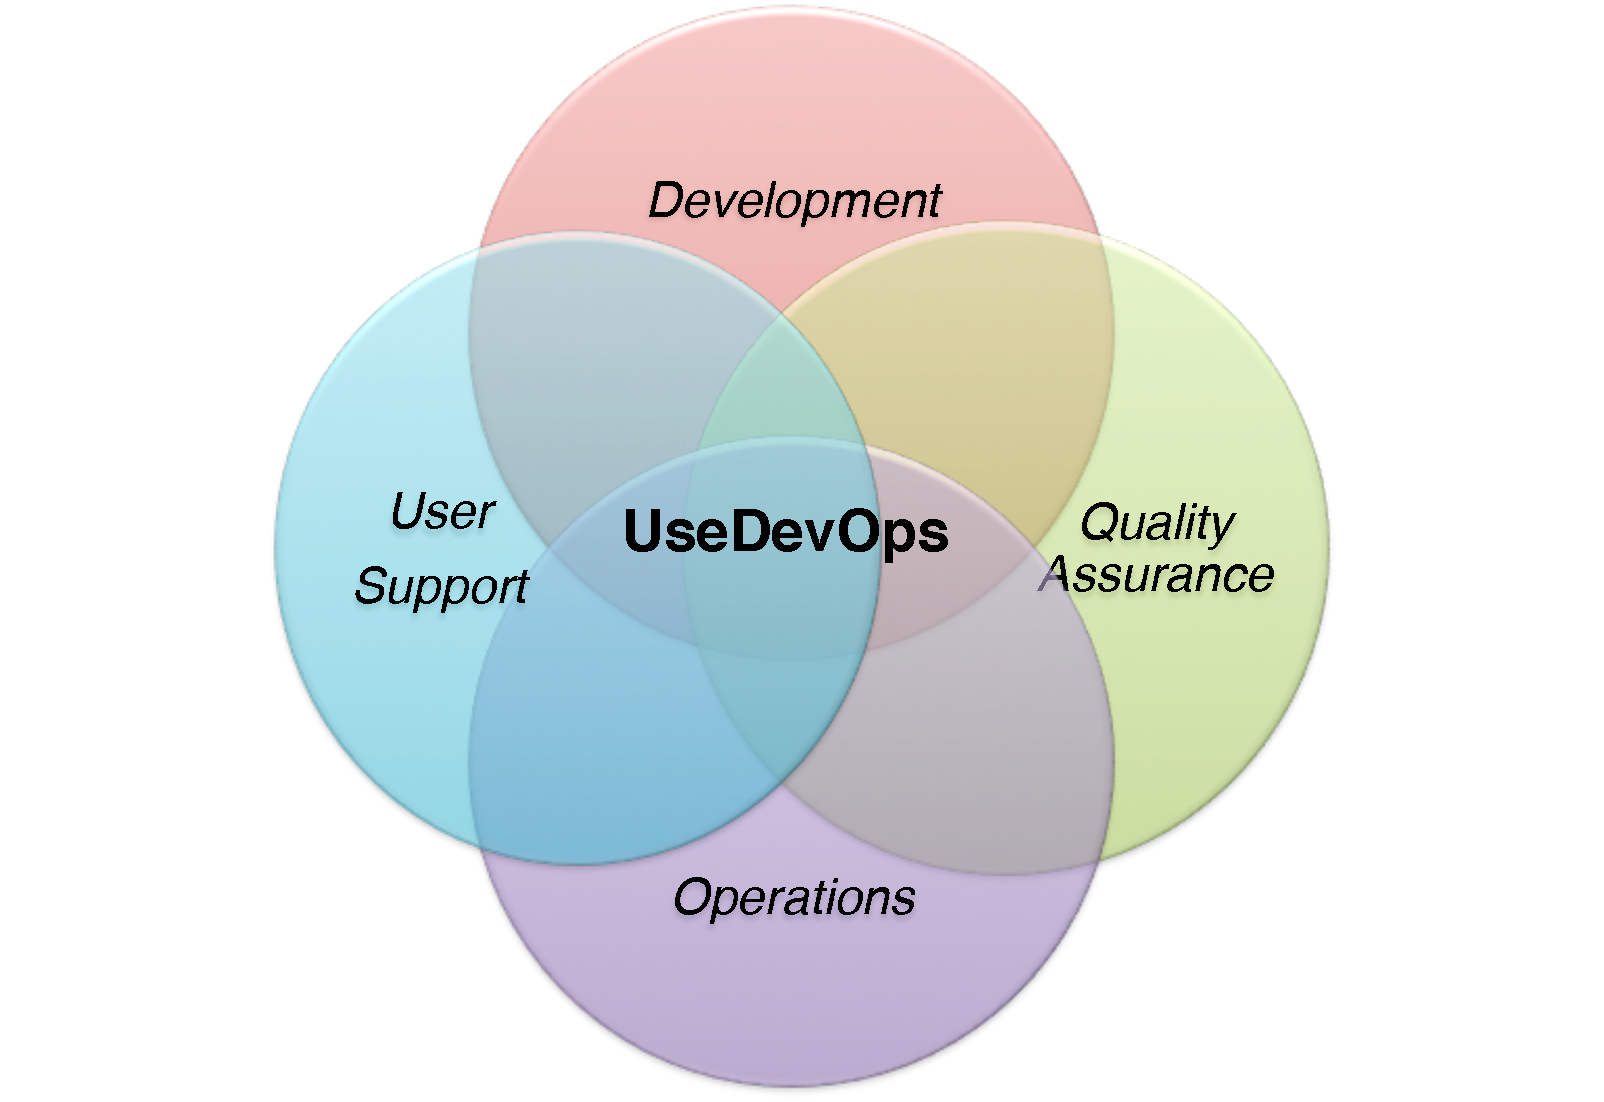
\includegraphics[width=0.5\textwidth]{images/usedevops.pdf}
  \caption{User Support integrated into DevOps leads to UseDevops.}
  \label{F:usedevops}
\end{figure}








%http://en.wikipedia.org/wiki/DevOps



